% !TeX program = xelatex
% Standalone preview for the RQ1/RQ3 segment; style matches C3_Paper_Theory.tex.
\PassOptionsToPackage{quiet}{fontspec}
\PassOptionsToPackage{dvipsnames}{xcolor}
\PassOptionsToPackage{fontset=fandol}{ctex}
\documentclass[10pt,aspectratio=169]{beamer}

\usepackage{zju_beamer}
\usepackage{booktabs}
\usepackage{tabularx}
\usepackage{array}
\usepackage{mathtools}

\graphicspath{{./figures/}{../../results/figures/}{../../docs/assets/}}
\zjusectioncolor{blue}
\setbeamertemplate{navigation symbols}{}

\definecolor{ZJUBlue}{RGB}{0,63,136}
\definecolor{ZJULight}{RGB}{236,244,252}
\definecolor{ZJUGreen}{RGB}{0,125,117}
\definecolor{WarmGray}{RGB}{90,90,90}
\newcommand{\key}[1]{\textcolor{ZJUBlue}{\textbf{#1}}}
\newcommand{\good}[1]{\textcolor{ZJUGreen}{\textbf{#1}}}

\title[C3：RQ1 与 RQ3]{数据增强 AutoML 市场：RQ1 与 RQ3}
\subtitle{发现算法与先验学习的论文实验及缩减复现}
\author[RQ1/RQ3 实验复现]{课程大作业 C.3 · RQ1/RQ3 实验复现部分}
\institute[数据要素市场]{数据要素市场课程 · 中期答辩\\参考论文：\textit{Optimal Pricing for Data-Augmented AutoML Marketplaces}}
\date{2026 年 7 月 18 日}

\begin{document}
\begin{frame}
  \titlepage
\end{frame}

% ============================================================
% RQ1 & RQ3 幻灯片 — 可直接插入 ZBY 的 Beamer 主文件
% 依赖：zju_beamer.sty、ZJUBlue/ZJUGreen、\key/\good 宏
% 图片搜索路径需包含 results/figures 与 docs/assets
% ============================================================

\providecommand{\slideref}[1]{\textcolor{black!60}{\small [#1]}}

% The combined deck defines all three switches.  The focused wrappers define
% only one RQ switch, so the same source can produce either RQ deck.

\section{RQ1：增强--模型发现}
\ifdefined\showrqone

\begin{frame}{RQ1：研究问题}
\begin{columns}[T,onlytextwidth]
\column{0.55\textwidth}
\begin{block}{研究问题}
在有限训练预算下，Data-Bandit 能否更早发现高质量的增强--模型组合？
\end{block}
\begin{block}{研究对象}
外部数据增强与机器学习模型的联合搜索。
\end{block}
\column{0.40\textwidth}
\begin{block}{评价维度}
\begin{itemize}
  \item 发现曲线与最终效用
  \item AUC
  \item 95\% oracle 增益训练次数
\end{itemize}
\end{block}
\end{columns}
\begin{alertblock}{核心比较}
Data-Bandit、Data-All、Data-Alt 与 AutoML。
\end{alertblock}
\end{frame}

\begin{frame}{RQ1：Algorithm 2}
\slideref{Data-Bandit：增强候选搜索与 Exp3 模型选择}
\begin{columns}[T,onlytextwidth]
\column{0.56\textwidth}
\begin{block}{算法步骤}
\begin{enumerate}
  \item 增强层提出候选 $T_i$；
  \item 按 Exp3 概率抽取一个模型 $M_i$；
  \item 只训练 $M_i\leftarrow(D_{\rm in}\Join T_i)$，得到奖励 $r_i$；
  \item 用重要性加权 $r_i/p_i(M_i)$ 更新模型权重。
\end{enumerate}
\end{block}
\begin{exampleblock}{训练预算}
与其在一个增强上花 $|\mathcal M|$ 次训练测透，不如先花 1 次快速筛选，从而把预算用于更多增强。
\end{exampleblock}
\column{0.41\textwidth}
\begin{block}{比较方法}
\small
\begin{itemize}
  \item \textbf{Data-Bandit：}每轮抽一个模型
  \item \textbf{Data-All：}每个增强训练全部模型
  \item \textbf{Data-Alt：}固定低成本模型筛增强，周期性完整搜模型
  \item \textbf{AutoML：}只搜模型，不加入外部数据
\end{itemize}
\end{block}
\begin{alertblock}{选择依据}
增强不断改变输入数据，模型奖励并非固定分布；Exp3 适合这种非平稳/对抗式反馈。
\end{alertblock}
\end{columns}
\end{frame}

\begin{frame}{RQ1：原文实验设计}
\slideref{原文 §6；Figure 3}
\begin{columns}[T,onlytextwidth]
\column{0.37\textwidth}
\begin{block}{原论文设置}
\small
\begin{itemize}
  \item 69K 个 NYC Open Data 数据集
  \item 约 30M 列、3B 行
  \item 1000 个分类/回归任务
  \item Random Forest、XGBoost、Neural Network 等
  \item 横轴：搜索时间；纵轴：效用
\end{itemize}
\end{block}
\column{0.61\textwidth}
\centering
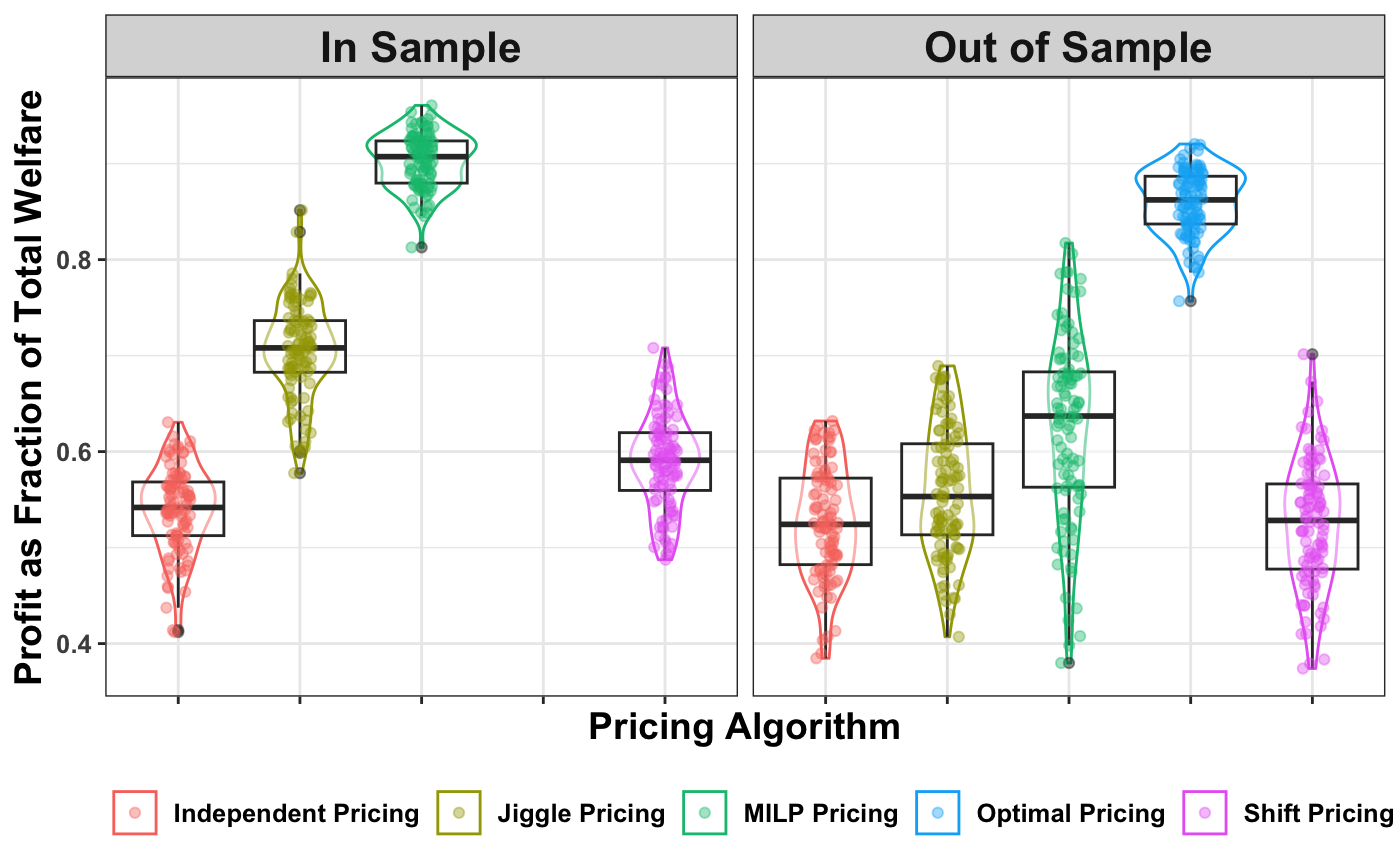
\includegraphics[width=\linewidth]{paper_rq1_figure3.png}
\vspace{0.2em}
{\scriptsize 原文 Figure 3；横轴为搜索时间，纵轴为效用。}
\end{columns}
\end{frame}

\begin{frame}{RQ1：原文实验结果}
\slideref{原文 Figure 3}
\begin{columns}[T,onlytextwidth]
\column{0.48\textwidth}
\begin{exampleblock}{分类任务}
\begin{itemize}
  \item Data-Bandit 平均效用超过 $0.85$
  \item 次优方法平均效用略高于 $0.70$
  \item AutoML 约为 $0.55$
\end{itemize}
\end{exampleblock}
\column{0.48\textwidth}
\begin{exampleblock}{回归任务}
\begin{itemize}
  \item Data-Bandit 在固定时间点均高于基线
  \item 多数任务识别出的增强数少于 10
  \item 结论：更高的有限时间发现效率
\end{itemize}
\end{exampleblock}
\end{columns}
\begin{alertblock}{原文结论}
Data-Bandit 在相同搜索时间下更快获得高质量增强--模型组合。
\end{alertblock}
\end{frame}

\begin{frame}{RQ1：复现实验设计}
\slideref{UCI Wine Quality；训练调用次数作为成本代理}
\begin{columns}[T,onlytextwidth]
\column{0.48\textwidth}
\begin{block}{数据与搜索空间}
\begin{itemize}
  \item 红/白葡萄酒，分类与回归各 30 个任务
  \item 2 个基础特征 + 9 个外部增强
  \item 6 个自包含模型族
  \item 每种方法最多 60 次模型训练
  \item 固定种子；每任务 60/20/20 划分
\end{itemize}
\end{block}
\column{0.50\textwidth}
\begin{block}{数据划分}
\begin{itemize}
  \item 训练集：排序增强候选、拟合模型
  \item 验证集：搜索与选择当前 incumbent
  \item 测试集：只报告验证选择方案的效用
\end{itemize}
\end{block}
\begin{alertblock}{复现边界}
NYC 数据池、Metam 配置和完整代码未公开；这里复现\textbf{预算语义和定性现象}，不逐点还原原图时间轴。
\end{alertblock}
\end{columns}
\end{frame}

\begin{frame}{RQ1：复现实验结果}
\centering
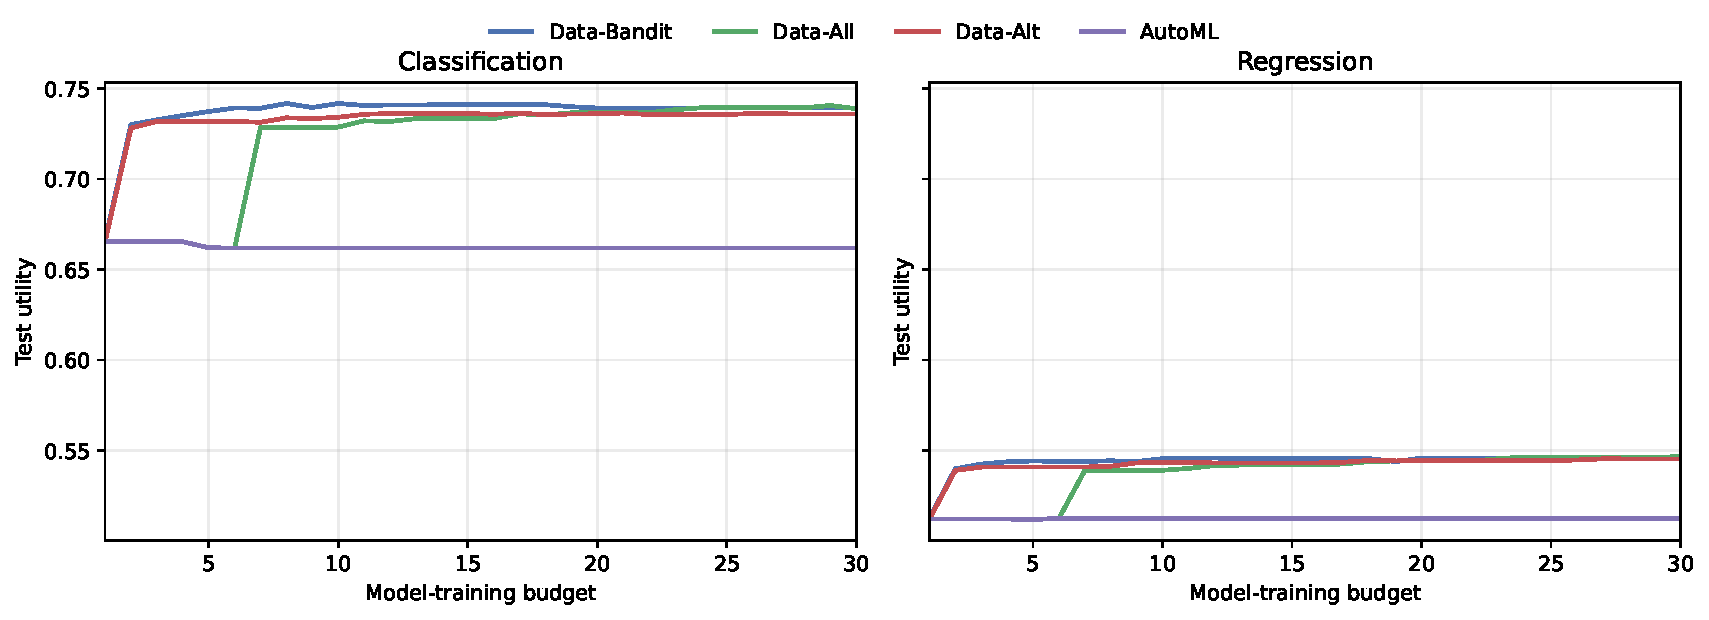
\includegraphics[width=0.86\linewidth]{rq1_discovery.pdf}
\vspace{-0.35em}
\begin{columns}[T,onlytextwidth]
\column{0.48\textwidth}
\begin{exampleblock}{搜索效率}
\small
\begin{itemize}
  \item AUC 配对差：分类 $+0.00794$，回归 $+0.00335$
  \item 95\% bootstrap 区间均不跨 0
  \item 达到 95\% oracle 增益所需训练减少 30.3\% / 27.5\%
\end{itemize}
\end{exampleblock}
\column{0.50\textwidth}
\begin{alertblock}{结果边界}
\small
\begin{itemize}
  \item 60 次预算终点仍是 Data-All 略高，差距 0.0012--0.0015
\item Bandit 与 Data-Alt 的 AUC 区间跨 0，只能说表现相当
\end{itemize}
\end{alertblock}
\end{columns}
\vspace{0.2em}
{\scriptsize 数据落盘：\texttt{results/tables/rq1\_task\_results.csv}、\texttt{rq1\_paired\_comparisons.csv}、\texttt{results/rq1\_summary.json}。}
\end{frame}
\fi

\ifdefined\showrqthree
\section{RQ3：先验学习}

\begin{frame}{RQ3：研究问题}
\slideref{先验学习与停止行为}
\begin{columns}[T,onlytextwidth]
\column{0.54\textwidth}
\begin{block}{研究问题}
平台未知买家类型先验时，能否仅凭停止轮次学习真实分布 $\mu^*$？
\end{block}
\begin{block}{观测变量}
买家在给定价格曲线与搜索过程下的停止轮次 $Y$。
\end{block}
\column{0.43\textwidth}
\begin{block}{评价指标}
\begin{itemize}
  \item $D_{\rm KL}(\mu^*\|\mu^{(t)})$
  \item 学习率对收敛速度的影响
  \item 批量对估计稳定性的影响
\end{itemize}
\end{block}
\begin{alertblock}{识别条件}
不同买家类型必须产生可区分的停止分布。
\end{alertblock}
\end{columns}
\end{frame}

\begin{frame}{RQ3：Algorithm 1}
\slideref{Bayesian Learning of Market's Prior Knowledge}
\begin{columns}[T,onlytextwidth]
\column{0.54\textwidth}
\begin{block}{算法步骤}
\begin{enumerate}
  \item 对每类 $\theta_i$ 预计算停止似然
  \[
  L_i(y)=\Pr(Y=y\mid\theta_i,x);
  \]
  \item 观察停止轮次 $y^{(t)}$ 后做 Bayes 更新
  \[
  w_i^{(t)}=\frac{L_i(y^{(t)})\mu_i^{(t)}}{\sum_jL_j(y^{(t)})\mu_j^{(t)}};
  \]
  \item 用学习率平滑
  \[
  \mu^{(t+1)}=(1-\eta_t)\mu^{(t)}+\eta_t\bar w^{(t)}.
  \]
\end{enumerate}
\end{block}
\column{0.43\textwidth}
\begin{block}{比较维度}
\begin{itemize}
  \item 真实先验 $\mu^*$ 的收敛性
  \item 学习率与收敛速度、波动
  \item 批量与估计稳定性
\end{itemize}
\end{block}
\begin{alertblock}{理论前提}
不同类型必须产生可区分的停止分布；否则只看停止轮次不可能区分它们。
\end{alertblock}
\end{columns}
\end{frame}

\begin{frame}{RQ3：原文实验设计}
\slideref{原文 §6；Figure 5；Appendix D.2}
\begin{columns}[T,onlytextwidth]
\column{0.35\textwidth}
\begin{block}{原论文设置}
\small
\begin{itemize}
  \item $|\mathcal Q|=10$，类型数 $n=5$，$T=15$
  \item 5 种先验：随机、均匀、略偏、高偏、极偏
  \item 学习率：$1/(t+1)$、$1/\sqrt t$、$1/2$
  \item 批量：10 与 100
  \item 指标：$D_{\rm KL}(\mu^*\|\mu^{(t)})$
\end{itemize}
\end{block}
\column{0.63\textwidth}
\centering
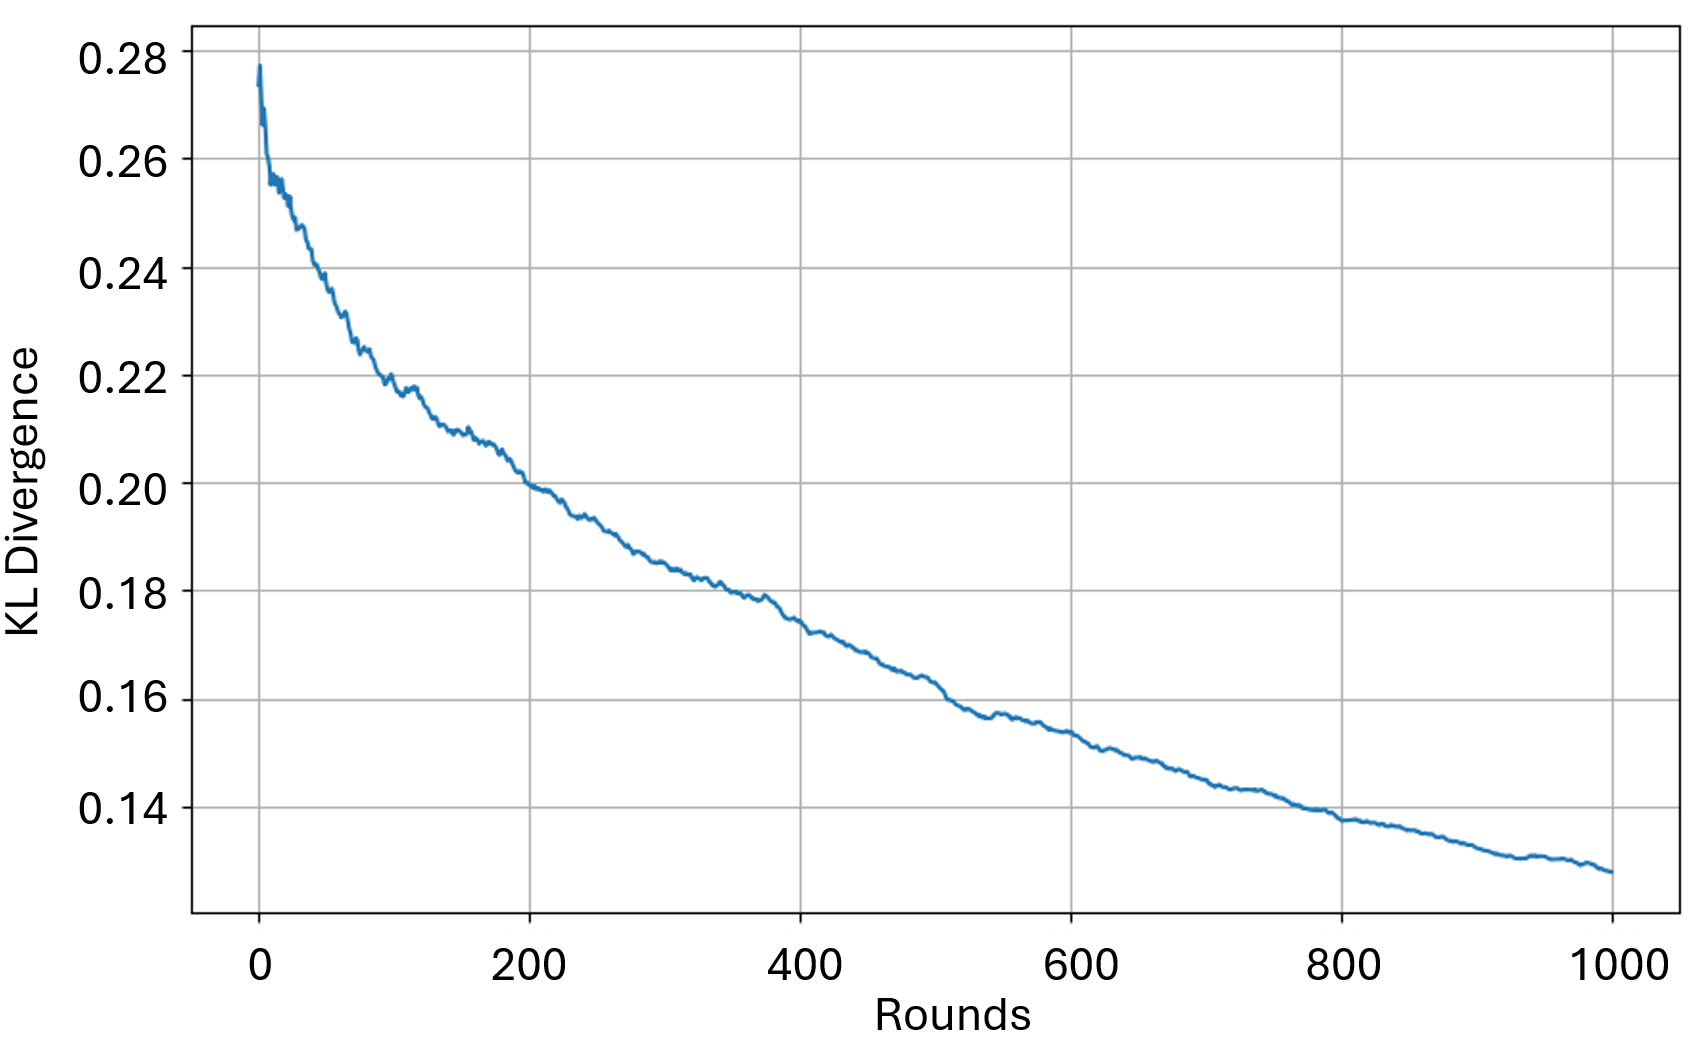
\includegraphics[width=0.32\linewidth]{paper_rq3_fig5_a.png}\hfill
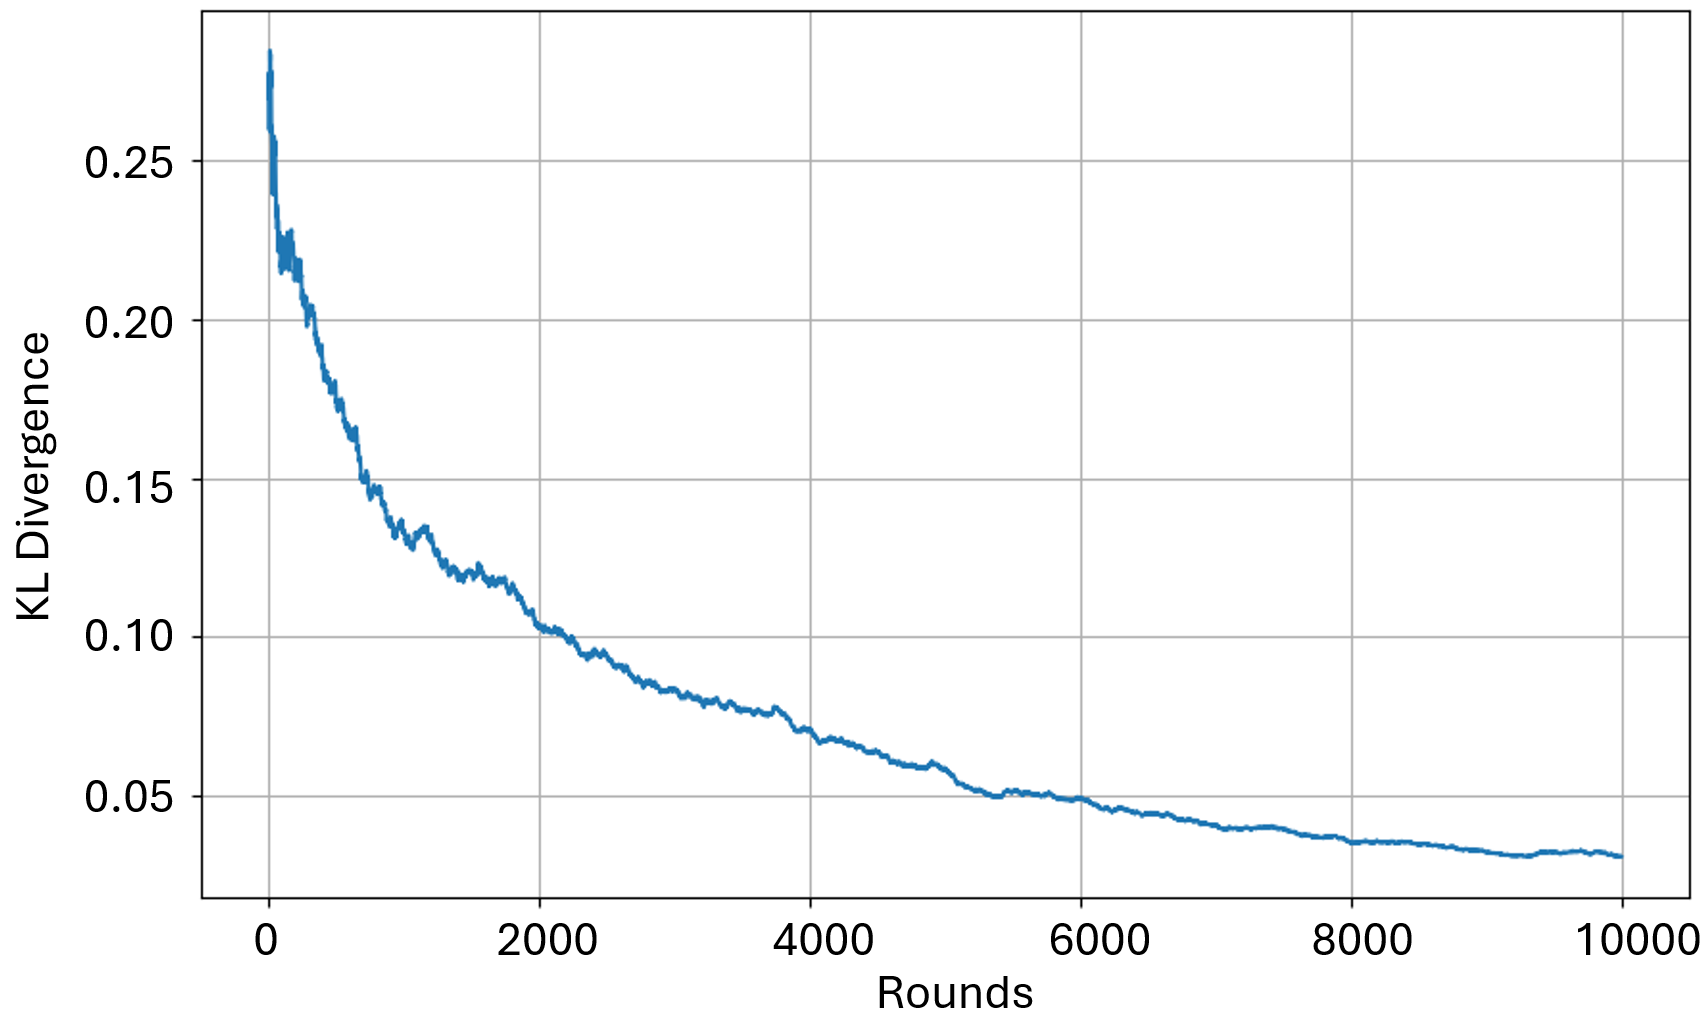
\includegraphics[width=0.32\linewidth]{paper_rq3_fig5_b.png}\hfill
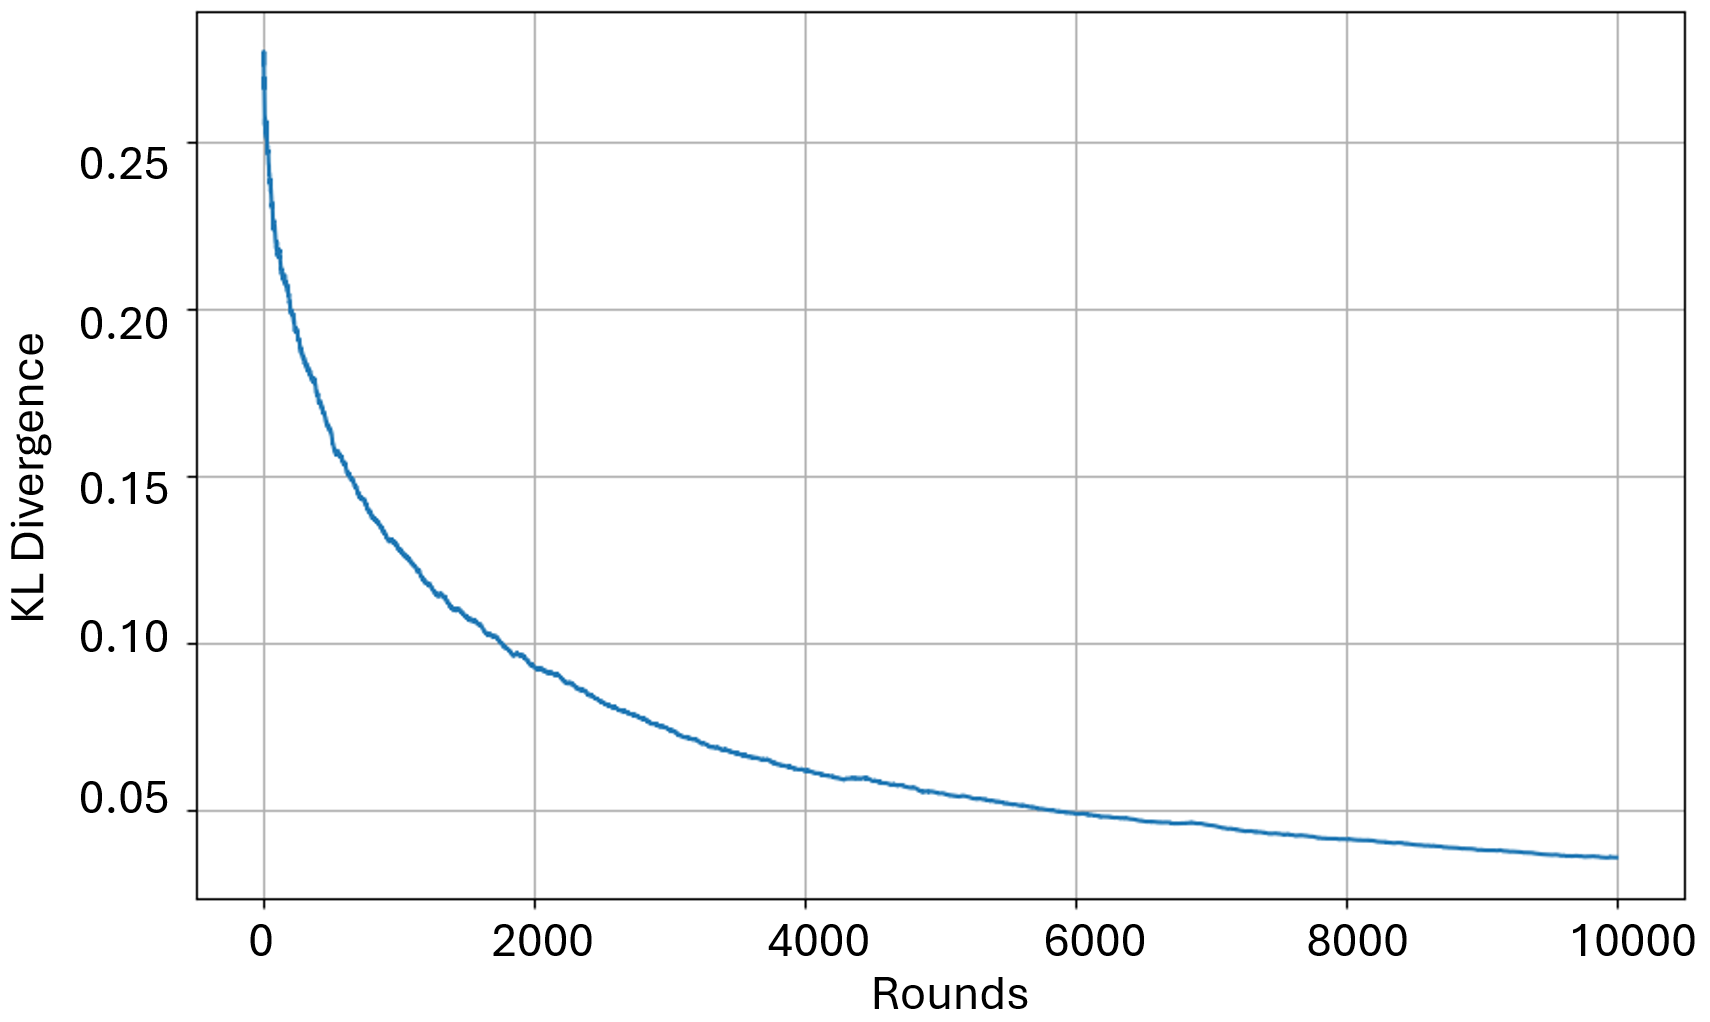
\includegraphics[width=0.32\linewidth]{paper_rq3_fig5_c.png}
\vspace{0.25em}
{\scriptsize Figure 5：(a) $b=100,1000$ 轮；(b) $b=10,10000$ 轮；(c) $b=100,10000$ 轮。}
\end{columns}
\end{frame}

\begin{frame}{RQ3：原文实验结果}
\slideref{原文 Figure 5；Appendix D.2}
\begin{columns}[T,onlytextwidth]
\column{0.48\textwidth}
\begin{exampleblock}{收敛结果}
\begin{itemize}
  \item KL 散度随学习轮次下降
  \item $1/\sqrt t$ 与 $1/2$ 收敛较快
  \item $1/(t+1)$ 收敛较慢但更平稳
\end{itemize}
\end{exampleblock}
\column{0.48\textwidth}
\begin{exampleblock}{批量效应}
\begin{itemize}
  \item 批量 100 的曲线更平滑
  \item 批量 10 的常数学习率波动更大
  \item 结果支持速度--稳定性权衡
\end{itemize}
\end{exampleblock}
\end{columns}
\begin{alertblock}{原文结论}
学习率与批量共同决定先验学习的收敛速度和稳定性。
\end{alertblock}
\end{frame}

\begin{frame}{RQ3：复现实验设计}
\slideref{透明合成 Markov 环境；精确停止似然}
\begin{columns}[T,onlytextwidth]
\column{0.49\textwidth}
\begin{block}{环境与似然}
\begin{itemize}
  \item 10 个质量状态、最长 15 轮
  \item 转移：52\% 停留、34\% 升一级、14\% 升两级
  \item 精确前向 DP 计算停止似然
  \item 五类估值 + 发现成本 0.018
\end{itemize}
\end{block}
\column{0.49\textwidth}
\begin{block}{实验组合}
\begin{itemize}
  \item 平均停止轮次：1.0、4.0、7.2、10.2、12.6
  \item 最小成对 $L_1$ 距离约 0.656
  \item 5 种先验 $\times$ 3 种学习率
  \item 批量 10/100、5 个种子、1000 轮
  \item 共 150 条学习运行
\end{itemize}
\end{block}
\begin{alertblock}{可识别性控制}
如果五类停止分布重合，学习失败可能只是不可识别，而不是 Algorithm 1 本身的问题。
\end{alertblock}
\end{columns}
\end{frame}

\begin{frame}{RQ3：复现实验结果}
\centering
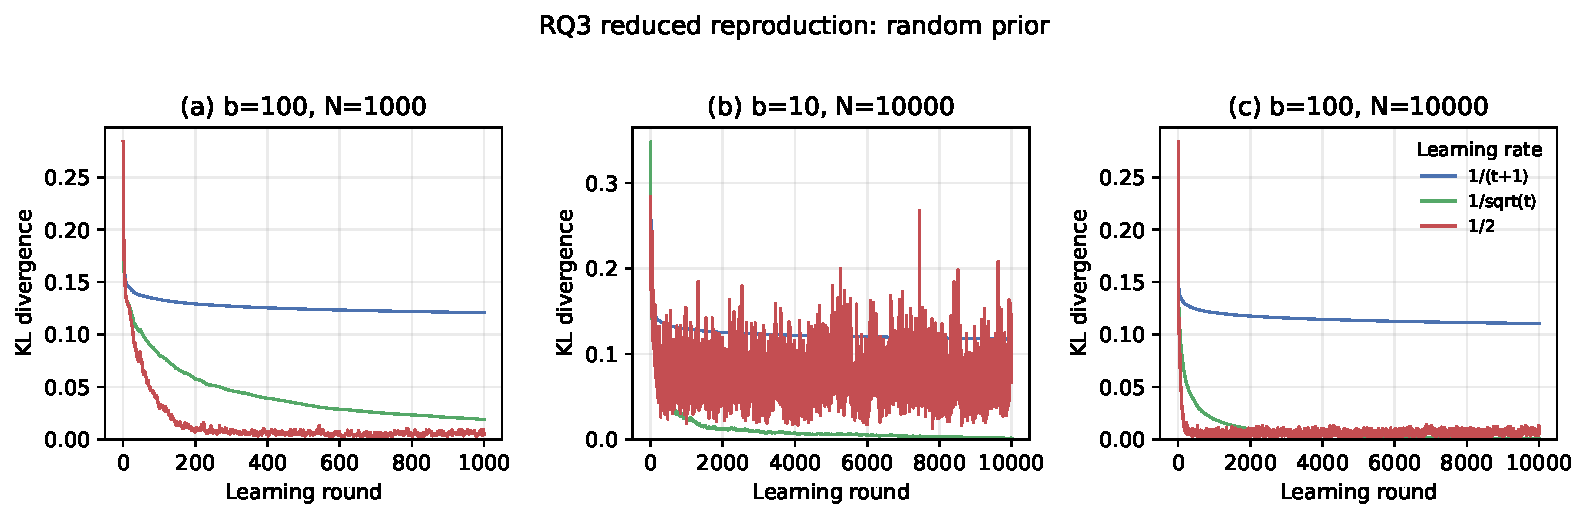
\includegraphics[height=0.47\textheight,keepaspectratio]{rq3_paper_reproduction.pdf}
\vspace{-0.3em}
\begin{columns}[T,onlytextwidth]
\column{0.48\textwidth}
\begin{exampleblock}{随机先验，批量 100}
\small
\begin{itemize}
  \item 最终 KL（$1/(t+1),1/\sqrt t,1/2$）：0.05185、0.00798、0.00702
  \item $1/2$ 最快，但尾部波动 0.00358
  \item $1/\sqrt t$ 的尾部波动仅 0.00032
\end{itemize}
\end{exampleblock}
\column{0.50\textwidth}
\begin{alertblock}{结果解释}
\small
\begin{itemize}
  \item $1/(t+1)$：最稳，但过早变得保守
  \item $1/2$：快，但持续受批次噪声影响
  \item $1/\sqrt t$：速度--稳定性折中
\item 批量 10 + 常数率时明显失稳
\end{itemize}
\end{alertblock}
\end{columns}
\vspace{0.2em}
{\scriptsize 数据落盘：\texttt{results/tables/rq3\_paper\_reproduction.csv}、\texttt{rq3\_paper\_summary.csv}、\texttt{results/paper\_experiments\_summary.json}；图由 \texttt{results/figures/rq3\_paper\_reproduction.pdf} 生成。}
\end{frame}
\fi

\ifdefined\showall
\begin{frame}{结论与复现边界}
\begin{columns}[T,onlytextwidth]
\column{0.48\textwidth}
\begin{exampleblock}{RQ1：发现效率}
\begin{itemize}
  \item Data-Bandit 以更少训练更早接近 oracle
  \item 相比 Data-All，AUC 差显著为正
  \item 但完整预算 Data-All 略高
  \item 相比 Data-Alt 只能说表现相当
\end{itemize}
\end{exampleblock}
\column{0.50\textwidth}
\begin{exampleblock}{RQ3：先验学习}
\begin{itemize}
  \item Algorithm 1 能在可识别环境中收敛
  \item 激进学习率更快但更易振荡
  \item 大批量可平滑抽样噪声
  \item $1/\sqrt t$ 是较均衡的折中
\end{itemize}
\end{exampleblock}
\end{columns}
\begin{alertblock}{统一的复现定位}
RQ1 使用 UCI 替代 NYC 数据池；RQ3 使用合成 Markov 环境。两者复现的是算法语义与定性结论，\textbf{不是 Figure 3/5 的逐点重现}。
\end{alertblock}
\end{frame}
\fi

\ifdefined\showall
\section*{备查页}

\begin{frame}{备查 A：Exp3 的概率与重要性加权}
\begin{block}{抽样概率}
\[
p_i(M)=(1-\gamma)\frac{w_i(M)}{\sum_{M'}w_i(M')}+\frac{\gamma}{|\mathcal M|}.
\]
\end{block}
\begin{columns}[T,onlytextwidth]
\column{0.49\textwidth}
\begin{block}{奖励估计}
只观察抽中模型 $M_i$：
\[
\widehat r_i(M_i)=\frac{r_i}{p_i(M_i)}.
\]
小概率抽到却高奖励，获得更强修正。
\end{block}
\column{0.49\textwidth}
\begin{block}{权重更新}
\[
w_{i+1}(M_i)=w_i(M_i)\exp\!\left(\frac{\gamma\widehat r_i(M_i)}{|\mathcal M|}\right).
\]
其他模型权重本轮不变。
\end{block}
\end{columns}
\begin{alertblock}{解释}
除以抽样概率是为了校正不同模型被观察频率不同造成的偏差；均匀探索项防止某只臂永远失去机会。
\end{alertblock}
\end{frame}

\begin{frame}{备查 B：RQ1 指标}
\small
\begin{enumerate}
  \item \textbf{final utility：}预算用尽时的测试效用，回答“最后谁最好”。
  \item \textbf{AUC：}$B^{-1}\sum_{b=1}^{B}U_b$，衡量搜索过程效率。字段名中的 normalized 指除以预算长度，不是除以 oracle。
  \item \textbf{达到 95\% oracle 增益的训练数：}
  \[
  \min\{b:U_b\ge U_0+0.95\max(0,U^*-U_0)\}.
  \]
  \item \textbf{配对 bootstrap：}同一任务上先做方法差，再重采样任务；区间跨 0 就不能声称显著差异。
\end{enumerate}
\begin{alertblock}{解释边界}
AUC 显著更高不等于最终性能显著更高；“更快接近最优”和“最终绝对最优”是两个问题。
\end{alertblock}
\end{frame}

\begin{frame}{备查 C：RQ3 关键数字与可识别性}
\begin{table}
\centering
\small
\begin{tabular}{lrrr}
\toprule
学习率 & 最终 KL & 尾部平均 KL & 尾部标准差\\
\midrule
$1/(t+1)$ & $0.05185\pm0.01235$ & 0.05214 & \textbf{0.00019}\\
$1/\sqrt t$ & $0.00798\pm0.00316$ & 0.00834 & 0.00032\\
$1/2$ & \textbf{$0.00702\pm0.00266$} & \textbf{0.00716} & 0.00358\\
\bottomrule
\end{tabular}
\end{table}
\begin{columns}[T,onlytextwidth]
\column{0.48\textwidth}
\begin{block}{批量 10 的警告}
常数 $1/2$ 在五种先验上的平均最终 KL 约 0.1965，尾部波动约 0.0488。
\end{block}
\column{0.50\textwidth}
\begin{alertblock}{可识别性}
若两类买家在所有可用价格下产生相同停止分布，仅凭停止时间无法区分；应引入更多信号或将其合并为有效类型。
\end{alertblock}
\end{columns}
\end{frame}
\fi

\end{document}
